\documentclass[hide notes,intlimits,usenames,dvipsnames]{beamer}

\mode<presentation>
{
  \usetheme{Singapore}
  \usefonttheme{professionalfonts}
  \setbeamertemplate{blocks}[rounded][shadow=true]
  \setbeamercovered{transparent}
  \setbeamertemplate{footline}[frame number]
}

% load packages
\usepackage[english]{babel}
\usepackage[latin1]{inputenc}
\usepackage[T1]{fontenc}
\usepackage{lmodern}
\usepackage[multidot]{grffile}
\usepackage{verbatim,empheq}

\usepackage{tikz}
\usetikzlibrary{shapes,arrows,shadows}
\usetikzlibrary{decorations.pathreplacing}

\usepackage{animate}
\usepackage{amsmath,verbatim}

% see http://tex.stackexchange.com/questions/86188/labelling-with-arrows-in-an-automated-way

\newif\ifclipme\clipmetrue
\tikzset{labelstyle/.style={LabelStyle/.append style={#1}},linestyle/.style={LineStyle/.append style={#1}}}
\tikzset{LabelStyle/.initial={},LineStyle/.initial={}}

\newcommand{\mathWithDescription}[4][]{{%
    \tikzset{#1}%
    \tikz[baseline]{
        \node[draw=red,rounded corners,anchor=base] (m#4) {$\displaystyle#2$};
        \ifclipme\begin{pgfinterruptboundingbox}\fi
            \node[above of=m#4,font=\strut, LabelStyle] (l#4) {#3};
            \draw[-,red, LineStyle] (l#4) to (m#4);
        \ifclipme\end{pgfinterruptboundingbox}\fi
    }%
}}

\newcommand{\mathWithDescriptionStarred}[3][]{{%
    \clipmefalse%
    \mathWithDescription[#1]{#2}{#3}{\themathLabelNode}%
}}

\newcounter{mathLabelNode}

\newcommand{\mathLabelBox}[3][]{%
   \stepcounter{mathLabelNode}%
   \mathWithDescription[#1]{#2}{#3}{\themathLabelNode}%
   \vphantom{\mathWithDescriptionStarred[#1]{#2}{#3}{\themathLabelNode}}%
}

\definecolor{dark red}{HTML}{E41A1C}
\definecolor{dark green}{HTML}{4DAF4A}
\definecolor{dark violet}{HTML}{984EA3}
\definecolor{dark blue}{HTML}{084594}
\definecolor{dark orange}{HTML}{FF7F00}
\definecolor{light blue}{HTML}{377EB8}
\definecolor{light red}{HTML}{FB9A99}
\definecolor{light violet}{HTML}{CAB2D6}

\newcommand{\CC}{\mathbb{C}}
\newcommand{\NN}{\mathbb{N}}
\newcommand{\RR}{\mathbb{R}}
\newcommand{\ZZ}{\mathbb{Z}}

\newcommand{\Kcal}{\mathcal{K}}
\newcommand{\Xcal}{\mathcal{X}}

\newcommand{\bF}{\mathbf{F}}
\newcommand{\bQ}{\mathbf{Q}}
\newcommand{\bU}{\mathbf{U}}
\newcommand{\bX}{\mathbf{X}}

\newcommand{\bq}{\mathbf{q}}
\newcommand{\bu}{\mathbf{u}}
\newcommand{\bv}{\mathbf{v}}
\newcommand{\bx}{\mathbf{x}}

\newcommand{\Div}{\nabla\cdot}
\newcommand{\eps}{\epsilon}
\newcommand{\grad}{\nabla}
\newcommand{\lap}{\triangle}
\renewcommand{\bar}{\overline}

\newcommand{\ip}[2]{\ensuremath{\left<#1,#2\right>}}


\newenvironment{transbox}[1][]{%
\begin{tikzpicture}
\node[drop shadow,rounded corners,text width=\textwidth,fill=white, fill opacity=#1,text opacity=1] \bgroup
}{
\egroup;\end{tikzpicture}}


\title{Optimal solvers for partial differential equations}

\author[Bueler]{Ed Bueler}

\institute[UAF]{
  \scriptsize Dept of Mathematics and Statistics and Geophysical Institute \\

  University of Alaska Fairbanks
}

%\titlegraphic{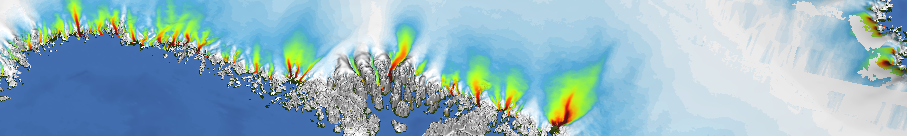
\includegraphics[width=\textwidth]{andycoast.png}}

\beamertemplatenavigationsymbolsempty   % remove faint and silly navigation symbols at bottom
\renewcommand{\insertnavigation}[1]{}   % remove section headings from top of each slide

\setbeamerfont{date}{size=\scriptsize}
\date{}

%\AtBeginSection[]
%{
%  \begin{frame}<beamer>
%    \frametitle{Outline}
%    %\tableofcontents[currentsection,hideallsubsections]
%    \tableofcontents[currentsection]
%  \end{frame}
%}


\begin{document}

%\graphicspath{{../../old/commonfigs/}}

\begin{frame}
\vspace{10mm}
  \titlepage
  \begin{center}
  \tiny DMS Colloquium \quad 28 November, 2017
  \end{center}
\end{frame}

  \begin{frame}
    \frametitle{Outline}
    \tableofcontents
  \end{frame}


\section{solving PDEs on a grid}

%\begin{frame}{ice sheet flows and their boundaries}
%\begin{columns}
%\begin{column}{0.45\textwidth}
%\begin{itemize}
%\item surface slope is discontinuous at grounded margins
%\end{itemize}
%\end{column}
%\begin{column}{0.55\textwidth}
%FIXME
%\end{column}
%\end{columns}
%\end{frame}


\begin{frame}{examples: Poisson and minimal surface equations}

\begin{itemize}
\item for most of this talk I'll use just two examples:
	\begin{itemize}

    \bigskip
	\item[$\circ$] \emph{Poisson equation} with Dirichlet boundary conditions:
	    $$- \grad^2 u = f \text{ on } \Omega \subset \RR^d \text{ with } u\big|_{\partial \Omega} = g,$$
	    \vspace{-5mm}
		\begin{itemize}
		\item linear problem
		\item $d=2,3$ and various $\Omega$
		\end{itemize}

    \bigskip
	\item[$\circ$] \emph{minimal surface equation (MSE)} with Dirichlet b.c.s:
	    $$- \grad\cdot \left(\frac{\grad u}{\sqrt{1 + |\grad u|^2}}\right) = 0  \text{ on } \Omega = [0,1]^2 \text{ with } u\big|_{\partial \Omega} = g.$$
	    \vspace{-2mm}
		\begin{itemize}
		\item nonlinear problem in 2D
		\end{itemize}
	\end{itemize}

\medskip
\item these are well-posed elliptic PDE problems
	\begin{itemize}
	\item[$\circ$] derived from variational principles
	\end{itemize}
\end{itemize}
\end{frame}


\begin{frame}{structured grids}
\begin{itemize}
\item for much of this talk I'll us \emph{structured grids} on $\Omega=[0,1]^d$
\item they will have various resolutions
	\begin{itemize}
	\item[$\circ$] denoted $\Omega^{(k)}$ where $k$ is the \emph{level}
    \item[$\circ$] the coarsest one under consideration is always $\Omega^{(0)}$
    \item[$\circ$] if we use $\Omega^{(0)},\Omega^{(1)},\dots,\Omega^{(k)}$ in a method then we call $\Omega^{(k)}$ \emph{the fine grid}
	\end{itemize}

\bigskip
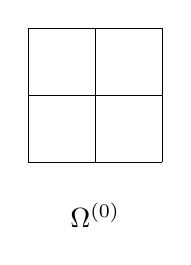
\begin{tikzpicture}[scale=1.7]
  \pgfmathsetmacro\half{1.0/2.0}
  \draw[xstep=\half,ystep=\half,black,thin] (0.0,0.0) grid (1.0,1.0);
  \node at (0.5,-0.4) {$\Omega^{(0)}$};
\end{tikzpicture}
\quad
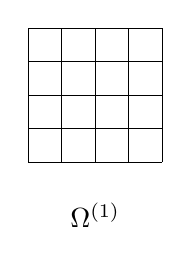
\begin{tikzpicture}[scale=1.7]
  \pgfmathsetmacro\fourth{1.0/4.0}
  \draw[xstep=\fourth,ystep=\fourth,black,thin] (0.0,0.0) grid (1.0,1.0);
  \node at (0.5,-0.4) {$\Omega^{(1)}$};
\end{tikzpicture}
\quad
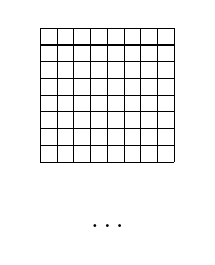
\begin{tikzpicture}[scale=1.7]
  \pgfmathsetmacro\eigth{1.0/8.0}
  \draw[xstep=\eigth,ystep=\eigth,black,thin] (0.0,0.0) grid (1.0,1.0);
  \node at (0.5,-0.4) {$\phantom{\Omega^{(2)}}\dots\phantom{\Omega^{(2)}}$};
\end{tikzpicture}
\quad
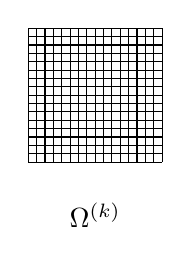
\begin{tikzpicture}[scale=1.7]
  \pgfmathsetmacro\sixteenth{1.0/16.0}
  \draw[xstep=\sixteenth,ystep=\sixteenth,black,thin] (0.0,0.0) grid (1.0,1.0);
  \node at (0.5,-0.4) {$\Omega^{(k)}$};
\end{tikzpicture}
\end{itemize}
\end{frame}


\begin{frame}{approximation: finite differences}
\begin{itemize}
\item FIXME
\end{itemize}
\end{frame}


\begin{frame}{approximation: finite elements}
\begin{itemize}
\item FIXME
\end{itemize}
\end{frame}


\begin{frame}{FIXME}
\begin{itemize}
\item FIXME
\end{itemize}
\end{frame}


\section{what is an ``optimal solver''?}

\begin{frame}{define ``optimal''}
\begin{itemize}
\item FIXME
\end{itemize}
\end{frame}

\begin{frame}{example: solving tridiagonal matrices}
\begin{itemize}
\item FIXME
\end{itemize}
\end{frame}

\begin{frame}{non-example:  banded Gaussian elimination (2D,3D)}
\begin{itemize}
\item FIXME
\end{itemize}
\end{frame}

\begin{frame}{tangent: spectral methods}
\begin{itemize}
\item FIXME
\item spectral methods show that pursuit of optimality is \emph{not} the only good goal
\end{itemize}
\end{frame}

\begin{frame}{Krylov methods}
\begin{itemize}
\item FIXME
\end{itemize}
\end{frame}

\begin{frame}{rate of convergence of CG}
\begin{itemize}
\item FIXME
\end{itemize}
\end{frame}


\section{multigrid}

\begin{frame}{FIXME}
\begin{itemize}
\item FIXME
\end{itemize}
\end{frame}

\begin{frame}{FIXME}
\begin{itemize}
\item FIXME
\end{itemize}
\end{frame}

\begin{frame}{an optimality lemma}

conditions under which multgrid cycles as preconditioners for CG give optimal solver
\begin{itemize}
\item FIXME
\end{itemize}
\end{frame}


\section{nonlinear problems and unstructured grids}

\begin{frame}{FIXME}
\begin{itemize}
\item FIXME
\end{itemize}
\end{frame}



\section{parallel scaling, and barriers to optimality}

\begin{frame}{FIXME}
\begin{itemize}
\item FIXME
\end{itemize}
\end{frame}


\end{document}
